%\subsection{Introduction} \label{subsection:android-introduction}

Android is an open source mobile \gls{os} launched in 2007 and currently developed by Google.
It is based on the Linux kernel and targets touch screen devices as mobile devices or wearables.
The system is designed to run efficiently on battery powered devices with limited hardware and computational capacity.
Android's main hardware platform is the ARM architecture since these processors with their low power consumtion are often used in this scenario.
The following will give an quick overview over the architecture of Android and a deeper insight in the runtime powering Android.

\begin{figure}[h]
    \centering
    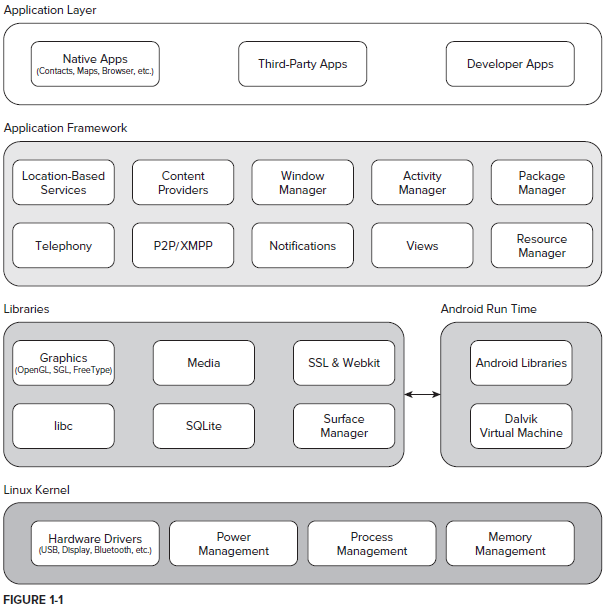
\includegraphics[width=0.8\textwidth]{data/stack.png}
    \caption{Android's architecture \cite{androidStack}}
    \label{fig:androidArchitecture}
\end{figure}

The architecture of the software stack of Android can be seen in figure~\ref{fig:androidArchitecture}.
\newline
The basis of the system is its kernel.
The kernel is responsible for power and memory management and is capable to execute standard Unix commands.
It provides an hardware abstraction layer for software and controls the device drivers.
\newline
The layer on top of the kernel contains \gls{art}, which will be explained in detail, as well as the the native libraries of the system.
Android libraries are usually written in Java except these native and speed critical ones.
They are written in C or C++ and allow low level interaction between applications and the kernel by using the \gls{jni}.
This includes libraries like OpenGL, multimedia playback or the SQLite database.
\newline
Above this layer is the application framework.
The application framework provides generic functionality as notification support to applications over Androids \gls{api}.
\newline
Applications are installed and executed on the top layer.
\newline
This structure enables Android to be run on a wide range of devices.



%The underlying entity of the system is its kernel which bridges the hardware of the device and the remaining software components. Being a Linux-based kernel, it allows remote access to the device via a Linux shell as well as the execution of standard Unix commands.
%Er ist für die Speicherverwaltung und Prozessverwaltung zuständig und stellt die Schnittstelle zum Abspielen von Multimedia und der Netzwerkkommunikation dar. Außerdem bildet er die Hardware-Abstraktionsschicht für den Rest der Software und stellt die Gerätetreiber für das System.

%A level above is the Android Runtime, which will be explained closer\newline
%At the same abstraction level as the virtual machine are the native libraries of the system. Written in C/C++, they permit low level interaction between the applications and the kernel through Java Native Interface (JNI)\newline
%The next layer is the application framework which provides generic functionality to mobile software through Android’s \gls{apig}.
%The top layer of the Android OS stack is where custom applications are compiled, installed and executed.\newline

%The top layer of the Android OS stack is where custom applications are compiled, in- stalled and executed. The file format of the install ready application is called Android Package (APK) and all the mobile software is distributed over Google Play in this for- mat. The APK format is a package management system based on the ZIP file archive format. Further details about the contents of Android applications are provided in the subsequent section.
%To show that Android is targeting a wide range of devices, including resource constrained ones, the minimal device hardware requirements [13] are given on table 1.1. Currently, most smartphones and tablets largely exceed the listed.

%\cite{kovachevaMaster}
%
